\chapter{\textbf{DNA Double Helix and Chromosome Compaction}\\[0.5cm]
	 Astonishing Parallels to T0-Torus Geometry\\[0.3cm]
	\normalsize From Molecular Winding to Highest Information Density}

	
	
\section*{Abstract}
		This paper examines the astonishing structural parallels between the DNA double helix, its hierarchical compaction into chromosomes, and the 4D torsional structure of T0 theory. The analysis reveals: Both systems use \textbf{the same geometric trick} -- \textbf{double helices winding around tori, which in turn fold hierarchically} -- to store maximum information in minimum volume. The study identifies \textbf{ten astonishing parallels}: (1) \textbf{Double helix as basic structure}, (2) \textbf{Winding numbers determine properties}, (3) \textbf{Hierarchical compaction across levels}, (4) \textbf{Toroidal geometry at each level}, (5) \textbf{Singularity avoidance through minimum radii}, (6) \textbf{Information maximization with volume minimization}, (7) \textbf{10,000-fold compression without loss}, (8) \textbf{Fractal self-similarity}, (9) \textbf{Topological stability}, (10) \textbf{Dynamic unfolding when needed}. DNA compaction is not an evolutionary accident, but rather the \textbf{biological solution to the same fundamental geometric problem} that also structures physics at all scales.

	
	
	
	\section{Introduction: The Packaging Problem}
	
	\subsection{DNA: 2 Meters in 6 $\mu$m}
	
	Every human cell faces an astonishing geometric problem:
	
	\begin{center}
		
		\textbf{How does one pack $\sim$2 meters of DNA into a nucleus of $\sim$6 $\mu$m diameter?}
	\end{center}
	
	This corresponds to a \textbf{compression factor of $\sim$10,000}!
	
	\subsection{T0: Universal Information in Space}
	
	T0 theory faces an analogous problem:
	
	\begin{center}
		
		\textbf{How does one encode maximum physical information in finite space without singularities?}
	\end{center}
	
	\subsection{The Common Solution}
	
	\begin{keyresult}[The Universal Principle]
		\textbf{Both use the same geometric strategy:}
		
		\vspace{0.3cm}
		
		\textbf{Double helices} $\to$ wind around \textbf{tori} $\to$ which \textbf{fold hierarchically} $\to$ and \textbf{dynamically unfold} when needed
		
		\vspace{0.3cm}
		
		This is the \textbf{optimal solution for information storage}!
	\end{keyresult}
	
	\section{The DNA Hierarchy}
	
	\subsection{Level 1: The Double Helix (Molecular)}
	
	\textbf{Structure}:
	\begin{itemize}
		\item Two antiparallel polynucleotide strands
		\item Right-handed helix
		\item Turn: 360° per 10.5 base pairs
		\item Diameter: $\sim$2 nm
		\item Pitch: $\sim$3.4 nm per turn
	\end{itemize}
	
	\textbf{Geometry}:
	\begin{equation}
		\text{Winding number } w = \frac{n_{\text{base pairs}}}{10.5} \approx \frac{L}{3.4\,\text{nm}}
	\end{equation}
	
	\subsection{Level 2: Nucleosomes (Histones)}
	
	\textbf{Structure}:
	\begin{itemize}
		\item DNA wraps 1.65 times around histone octamer
		\item Histone core diameter: $\sim$11 nm
		\item 147 base pairs per nucleosome
		\item "Beads on a string"
	\end{itemize}
	
	\textbf{Compression}: $\sim$6-fold
	
	\textbf{Geometry -- TORUS!}:
	\begin{equation}
		R_{\text{Histone}} \approx 5.5\,\text{nm}, \quad r_{\text{DNA}} \approx 1\,\text{nm}
	\end{equation}
	
	The DNA forms a \textbf{toroidal loop} around the histone core!
	
	\subsection{Level 3: 30-nm Fiber (Solenoid)}
	
	\textbf{Structure}:
	\begin{itemize}
		\item Nucleosome chain folds into \textbf{solenoid}
		\item 6 nucleosomes per turn
		\item Diameter: $\sim$30 nm
		\item "Fiber of fibers"
	\end{itemize}
	
	\textbf{Compression}: $\sim$40-fold (cumulative)
	
	\textbf{Geometry -- HELIX of TORI!}
	
	\subsection{Level 4: Higher Loops ($\sim$300 nm)}
	
	\textbf{Structure}:
	\begin{itemize}
		\item 30-nm fiber forms loops
		\item Loops attached to protein scaffold
		\item Diameter: $\sim$300 nm
	\end{itemize}
	
	\textbf{Compression}: $\sim$400-fold (cumulative)
	
	\subsection{Level 5: Condensed Chromatin}
	
	\textbf{Structure}:
	\begin{itemize}
		\item Further folding of loop domains
		\item Diameter: $\sim$700 nm
	\end{itemize}
	
	\textbf{Compression}: $\sim$1,000-fold (cumulative)
	
	\subsection{Level 6: Metaphase Chromosome (Maximum Compaction)}
	
	\textbf{Structure}:
	\begin{itemize}
		\item Highest condensation during cell division
		\item Length: $\sim$1--10 $\mu$m
		\item Diameter: $\sim$1 $\mu$m
		\item X-shaped structure (two sister chromatids)
	\end{itemize}
	
	\textbf{Compression}: $\sim$\textbf{10,000-fold}!
	
	\begin{center}
		\textbf{2 meters DNA $\to$ 6 $\mu$m nucleus}
	\end{center}
	
	\section{The T0 Hierarchy}
	
	\subsection{Level 1: Fundamental (Sub-Planck)}
	
	\textbf{Structure}: 4D torsional crystal
	\begin{itemize}
		\item Double loop -- analogous to DNA double strand
		\item Toroidal + poloidal circulation
		\item Winding number $w = n_\phi / n_\theta$
		\item Minimum radius: $r_{\min} = 21\ell_P$
	\end{itemize}
	
	\subsection{Level 2: Particles ($\sim 10^{-15}$ m)}
	
	\textbf{Structure}: Elementary particles as torus resonances
	\begin{itemize}
		\item Electrons, quarks = stable windings
		\item Toroidal structure on Compton scale
		\item Spin from winding number
	\end{itemize}
	
	\subsection{Levels 3--6: Scale-Invariant Hierarchy}
	
	Further torus structures on all scales up to cosmic:
	\begin{itemize}
		\item Atoms $\sim 10^{-10}$ m
		\item Planets $\sim 10^{6}$ m  
		\item Stars $\sim 10^{9}$ m
		\item Galaxies $\sim 10^{20}$ m
	\end{itemize}
	
	\textbf{Compression}: $\sim 60$ orders of magnitude with $D_f = 3-\xi$!
	
	\section{The Ten Astonishing Parallels}
	
	\subsection{Parallel 1: Double Helix as Basic Structure}
	
	\subsubsection{DNA}
	
	The \textbf{double helix} is the fundamental structure:
	\begin{itemize}
		\item Two strands wound around each other
		\item Right-handed
		\item Complementary (A-T, G-C)
		\item Stability through \textbf{both} strands
	\end{itemize}
	
	\subsubsection{T0}
	
	The electron model (Williamson \& van der Mark, 1997) shows \textbf{double helix / double loop}:
	\begin{itemize}
		\item Two circulations: toroidal + poloidal
		\item Circularly polarized field
		\item Winding over Compton wavelength $\lambda_C$
		\item Stability through \textbf{both} circulations
	\end{itemize}
	
	\begin{keyresult}[First Parallel]
		\textbf{Double Circulation / Double Helix}
		
		Both use \textbf{two intertwined components}:
		\begin{itemize}
			\item DNA: Two nucleotide strands
			\item T0: Toroidal + poloidal flow
		\end{itemize}
		
		The \textbf{factor 2} is fundamental for stability!
	\end{keyresult}
	
	\subsection{Parallel 2: Winding Numbers Determine Properties}
	
	\subsubsection{DNA}
	
	The \textbf{number of turns} determines:
	\begin{itemize}
		\item Helix length
		\item Number of base pairs
		\item Topological properties (linking number)
		\item Supercoiling behavior
	\end{itemize}
	
	\textbf{Example}: Plasmid with 4,000 base pairs has $\sim$380 helix turns
	
	\subsubsection{T0}
	
	The \textbf{winding number} $w = n_\phi / n_\theta$ determines:
	\begin{itemize}
		\item Spin: $w = 1/2$ $\to$ fermions
		\item Spin: $w = 1$ $\to$ bosons
		\item Charge from flux quantization
		\item Mass from resonance
	\end{itemize}
	
	\begin{keyresult}[Second Parallel]
		\textbf{Winding Number = Quantum Number}
		
		\vspace{0.3cm}
		
		\begin{center}
			\begin{tabular}{p{5cm}|p{5cm}}
				\toprule
				\textbf{DNA} & \textbf{T0} \\
				\midrule
				Number of turns determines length & Winding number determines spin \\
				Linking number topological & Winding number topological \\
				Supercoiling energy & Field energy \\
				\bottomrule
			\end{tabular}
		\end{center}
	\end{keyresult}
	
	\subsection{Parallel 3: Hierarchical Compaction}
	
	\subsubsection{DNA}
	
	\textbf{6 Hierarchy Levels}:
	
	\begin{center}
		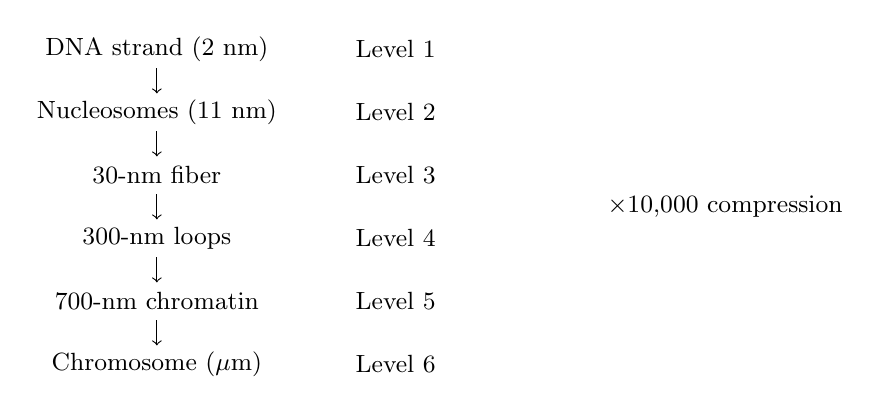
\begin{tikzpicture}[scale=0.8, every node/.style={font=\small}]
			\node at (0,6) {DNA strand (2 nm)};
			\draw[->] (0,5.7) -- (0,5.3);
			\node at (0,5) {Nucleosomes (11 nm)};
			\draw[->] (0,4.7) -- (0,4.3);
			\node at (0,4) {30-nm fiber};
			\draw[->] (0,3.7) -- (0,3.3);
			\node at (0,3) {300-nm loops};
			\draw[->] (0,2.7) -- (0,2.3);
			\node at (0,2) {700-nm chromatin};
			\draw[->] (0,1.7) -- (0,1.3);
			\node at (0,1) {Chromosome ($\mu$m)};
			
			\node[right] at (3,6) {Level 1};
			\node[right] at (3,5) {Level 2};
			\node[right] at (3,4) {Level 3};
			\node[right] at (3,3) {Level 4};
			\node[right] at (3,2) {Level 5};
			\node[right] at (3,1) {Level 6};
			
			\node[right, text width=3cm] at (7,3.5) {$\times$10,000 compression};
		\end{tikzpicture}
	\end{center}
	
	\subsubsection{T0}
	
	\textbf{60+ Hierarchy Levels}:
	
	From Sub-Planck ($10^{-39}$ m) to Cosmic ($10^{26}$ m)
	
	\begin{keyresult}[Third Parallel]
		Both use \textbf{hierarchical folding across multiple scales}:
		
		DNA: 6 levels, 10,000-fold compression
		
		T0: 60+ levels, self-similar with $D_f = 3-\xi$
	\end{keyresult}
	
	\subsection{Parallel 4: Toroidal Geometry}
	
	\subsubsection{DNA}
	
	\textbf{Torus at every level}:
	
	\textbf{Level 2 (Nucleosomes)}: DNA wraps \textbf{1.65 times around histone core}
	\begin{equation}
		\text{Torus}: R = 5.5\,\text{nm}, \quad r = 1\,\text{nm}
	\end{equation}
	
	\textbf{Level 3 (Solenoid)}: Nucleosome chain forms \textbf{helix} (torus-like)
	
	\textbf{Level 4+}: Loop domains attached to central axis = \textbf{toroidal arrangement}
	
	\subsubsection{T0}
	
	\textbf{Torus on EVERY scale}:
	\begin{itemize}
		\item Sub-Planck: Fundamental 4D torus
		\item Particles: Torus resonances
		\item Macro: Magnetic fields, plasmatoroids
		\item Cosmic: Galactic spirals, cosmic web
	\end{itemize}
	
	\begin{keyresult}[Fourth Parallel]
		\textbf{The torus is the universal geometry}
		
		Why? Because it:
		\begin{itemize}
			\item Is closed (no boundaries)
			\item Enables two independent circulations
			\item Stores energy/information efficiently
			\item Is topologically stable (genus = 1)
		\end{itemize}
	\end{keyresult}
	
	\subsection{Parallel 5: Singularity Avoidance}
	
	\subsubsection{DNA}
	
	\textbf{Minimum radii prevent collapse}:
	
	\begin{itemize}
		\item DNA helix cannot go below $\sim$1 nm radius
		\item Nucleosomes have fixed core diameter
		\item 30-nm fiber has minimum bending
		\item Too strong compression $\to$ DNA damage
	\end{itemize}
	
	\textbf{Reason}: Steric hindrance, Van der Waals radii, hydrogen bonds
	
	\subsubsection{T0}
	
	\textbf{Minimum torus radius}:
	\begin{equation}
		r_{\min} = 21\ell_P \approx 3.4 \times 10^{-34}\,\text{m}
	\end{equation}
	
	\textbf{Reason}: Fractal dimension $D_f = 3-\xi$ prevents singularity
	
	\begin{keyresult}[Fifth Parallel]
		\textbf{Both have fundamental lower limit}
		
		\begin{table}[H]
			\centering
			\begin{tabular}{lcc}
				\toprule
				& \textbf{DNA} & \textbf{T0} \\
				\midrule
				Minimum radius & $\sim$1 nm & $21\ell_P$ \\
				Cause & Chemical & Geometrical \\
				Consequence & DNA stability & No singularity \\
				\bottomrule
			\end{tabular}
		\end{table}
	\end{keyresult}
	
	\subsection{Parallel 6: Information Maximization}
	
	\subsubsection{DNA}
	
	\textbf{Problem}: 3 billion base pairs of information in $\sim$6 $\mu$m
	
	\textbf{Solution}: Hierarchical folding
	
	\textbf{Result}:
	\begin{itemize}
		\item Information density: $\sim 10^{9}$ bits / $\mu$m³
		\item Highest known information density in biology!
		\item Access when needed through local unfolding
	\end{itemize}
	
	\subsubsection{T0}
	
	\textbf{Problem}: Maximum physical information in finite space
	
	\textbf{Solution}: Fractal torus folding
	
	\textbf{Result}:
	\begin{itemize}
		\item Holographic principle: Information on surface
		\item Folding maximizes surface area
		\item Torus has maximum surface area for given volume
	\end{itemize}
	
	\begin{keyresult}[Sixth Parallel]
		\textbf{Both maximize} $\frac{\text{Information}}{\text{Volume}}$
		
		The folding is the \textbf{solution to an optimization problem}!
	\end{keyresult}
	
	\subsection{Parallel 7: Compression Factor}
	
	\subsubsection{DNA}
	
	\textbf{Quantitative}:
	\begin{align}
		\text{Stretched DNA} &: \sim 2\,\text{m} \\
		\text{Chromosome} &: \sim 6\,\text{µm} \\
		\text{Compression factor} &: \frac{2\,\text{m}}{6\,\text{µm}} \approx 333,000
	\end{align}
	
	Considering diameter: $\sim$\textbf{10,000-fold}
	
	\subsubsection{T0}
	
	\textbf{Quantitative}:
	\begin{align}
		\text{Planck scale} &: 10^{-35}\,\text{m} \\
		\text{Hubble scale} &: 10^{26}\,\text{m} \\
		\text{Orders of magnitude} &: 61
	\end{align}
	
	With $\xi = 1.33 \times 10^{-4}$: Scaling factor $\sim 1/\xi \approx 7500$ per level!
	
	\begin{keyresult}[Seventh Parallel]
		\textbf{Both achieve enormous compression without information loss}
		
		DNA: 10,000-fold (6 levels)
		
		T0: $7500^{60}$ (60 levels) = unimaginable!
	\end{keyresult}
	
	\subsection{Parallel 8: Fractal Self-Similarity}
	
	\subsubsection{DNA}
	
	\textbf{Self-similar structure}:
	\begin{itemize}
		\item Helix (Level 1) $\to$ winds into solenoid (helix of helices, Level 3)
		\item Nucleosomes (tori, Level 2) $\to$ arranged on helix (Level 3)
		\item 30-nm fiber $\to$ folds into loops (Level 4) $\to$ into chromatin (Level 5)
	\end{itemize}
	
	\textbf{Each level is a folded version of the previous one!}
	
	\subsubsection{T0}
	
	\textbf{Strict self-similarity}:
	\begin{equation}
		\frac{R_{\text{Level } n+1}}{R_{\text{Level } n}} = \frac{1}{\xi} \approx 7500
	\end{equation}
	
	The ratio $R/r$ remains constant across scales!
	
	\begin{keyresult}[Eighth Parallel]
		\textbf{Fractal repetition of the same pattern}
		
		DNA: Qualitatively self-similar (helix $\to$ solenoid $\to$ loops)
		
		T0: Quantitatively self-similar ($D_f = 3-\xi$, fixed scaling ratio)
	\end{keyresult}
	
	\subsection{Parallel 9: Topological Stability}
	
	\subsubsection{DNA}
	
	\textbf{Topological invariants}:
	
	\begin{itemize}
		\item \textbf{Linking number} (Lk): Number of intertwinings
		\item \textbf{Twist} (Tw): Local turns
		\item \textbf{Writhe} (Wr): Supercoiling
		
		Fundamental relationship:
		\begin{equation}
			\text{Lk} = \text{Tw} + \text{Wr}
		\end{equation}
	\end{itemize}
	
	These numbers are \textbf{topologically invariant} -- change only through cutting!
	
	\subsubsection{T0}
	
	\textbf{Topological quantum numbers}:
	\begin{itemize}
		\item Winding number $w = n_\phi / n_\theta$
		\item Flux quantization $\Phi = n \cdot h/e$
		\item Charge, spin, color charge from topology
	\end{itemize}
	
	These are \textbf{topologically protected} -- change only at phase transition!
	
	\begin{keyresult}[Ninth Parallel]
		\textbf{Topological stability}
		
		Both use \textbf{topological invariants} for stability:
		
		DNA: Linking number preserves structure
		
		T0: Winding number preserves quantum numbers
	\end{keyresult}
	
	\subsection{Parallel 10: Dynamic Unfolding}
	
	\subsubsection{DNA}
	
	\textbf{Unfolding when needed}:
	
	\begin{itemize}
		\item \textbf{Transcription}: Local unfolding for RNA polymerase
		\item \textbf{Replication}: Complete unfolding during S-phase
		\item \textbf{Recombination}: Temporary unfolding for repair
		\item \textbf{Regulation}: Acetylation $\to$ loose structure $\to$ accessibility
	\end{itemize}
	
	The compaction is \textbf{reversible} and \textbf{regulatable}!
	
	\subsubsection{T0}
	
	\textbf{Dynamic processes}:
	\begin{itemize}
		\item Energy flows in torus variable
		\item Torsion waves propagate
		\item Particle creation = excitation
		\item Phase transitions possible
	\end{itemize}
	
	The structure is \textbf{static}, but energy is \textbf{dynamic}!
	
	\begin{keyresult}[Tenth Parallel]
		\textbf{Static structure, dynamic processes}
		
		\vspace{0.3cm}
		
		\begin{center}
			\begin{tabular}{lcc}
				\toprule
				& \textbf{DNA} & \textbf{T0} \\
				\midrule
				Structure & Chromosome (static) & Torsion crystal (static) \\
				Dynamics & Local unfolding & Energy flows \\
				Reversible? & Yes & Yes (excitations) \\
				\bottomrule
			\end{tabular}
		\end{center}
	\end{keyresult}
	
	\section{Why These Parallels?}
	
	\subsection{Universal Optimization Problem}
	
	\begin{philosophical}[The Fundamental Question]
		Both biology (DNA) and physics (T0) face \textbf{the same challenge}:
		
		\vspace{0.3cm}
		
		\textbf{How does one store maximum information (sequence / physical states) in minimum space without:}
		\begin{itemize}
			\item Knotting (topology problems)
			\item Singularities (infinite energies)
			\item Information loss (entropy)
			\item Inaccessibility (must remain readable)
		\end{itemize}
		
		\vspace{0.3cm}
		
		The \textbf{answer is universal}: \textbf{Hierarchical torus folding with double helices}!
	\end{philosophical}
	
	\subsection{Mathematical Necessity}
	
	The parallels are not coincidental but follow from:
	
	\textbf{1. Topology}:
	\begin{itemize}
		\item Torus (genus = 1) is simplest non-trivial closed surface
		\item Enables two independent circulations
		\item Topologically stable
	\end{itemize}
	
	\textbf{2. Geometry}:
	\begin{itemize}
		\item Helix is natural curve in 3D
		\item Double helix maximizes stability
		\item Winding around torus is optimum
	\end{itemize}
	
	\textbf{3. Information theory}:
	\begin{itemize}
		\item Holographic principle: Information on surface
		\item Folding maximizes surface area
		\item Hierarchy allows logarithmic compression
	\end{itemize}
	
	\subsection{Evolution vs. Fundamentality}
	
	\begin{revolutionary}[The Deep Insight]
		\textbf{Did evolution "discover" torus geometry?}
		
		\vspace{0.3cm}
		
		\textbf{NO!}
		
		\vspace{0.3cm}
		
		Evolution \textbf{had to} use this geometry because it is the \textbf{only optimal solution} to the information storage problem!
		
		\vspace{0.3cm}
		
		Just as physics \textbf{had to} use the same geometry for fundamental structure!
		
		\vspace{0.3cm}
		
		DNA compaction is \textbf{not a random biological invention}, but rather the \textbf{manifestation of a universal geometric truth}!
	\end{revolutionary}
	
	\section{Quantitative Comparisons}
	
	\subsection{Compression Factors}
	
	\begin{table}[H]
		\centering
		\begin{tabular}{lccc}
			\toprule
			\textbf{System} & \textbf{From} & \textbf{To} & \textbf{Factor} \\
			\midrule
			DNA & 2 m & 6 $\mu$m & 333,000$\times$ \\
			& (stretched) & (chromosome) & \\
			T0 & $10^{-35}$ m & $10^{26}$ m & $10^{61}$ \\
			& (Sub-Planck) & (cosmic) & \\
			\bottomrule
		\end{tabular}
		\caption{Compression factors}
	\end{table}
	
	\subsection{Hierarchy Levels}
	
	\begin{table}[H]
		\centering
		\begin{tabular}{lccc}
			\toprule
			\textbf{System} & \textbf{Levels} & \textbf{Factor/Level} & \textbf{Geometry} \\
			\midrule
			DNA & 6 & $\sim$2--6$\times$ & Helix + Torus \\
			T0 & 60+ & $\sim$7500$\times$ & Torus + Fractal \\
			\bottomrule
		\end{tabular}
		\caption{Hierarchical structure}
	\end{table}
	
	\subsection{Characteristic Lengths}
	
	\begin{table}[H]
		\centering
		\small
		\begin{tabular}{llll}
			\toprule
			\textbf{DNA Level} & \textbf{Length} & \textbf{T0 Analog} & \textbf{Length} \\
			\midrule
			Double helix & 2 nm & Sub-Planck & $10^{-39}$ m \\
			Nucleosome & 11 nm & Particle & $10^{-15}$ m \\
			30-nm fiber & 30 nm & Atom & $10^{-10}$ m \\
			Loop & 300 nm & Molecule & $10^{-9}$ m \\
			Chromatin & 700 nm & Macro & $10^{0}$ m \\
			Chromosome & 1 $\mu$m & Cosmic & $10^{26}$ m \\
			\bottomrule
		\end{tabular}
		\caption{Scale comparison (qualitative)}
	\end{table}
	
	\section{Conclusion}
	
	\begin{keyresult}[Main Result]
		DNA compaction and T0 torus geometry show \textbf{ten astonishing structural parallels}:
		
		\vspace{0.3cm}
		
		\begin{enumerate}
			\item Double helix / Double circulation
			\item Winding numbers = quantum numbers
			\item Hierarchical compaction
			\item Toroidal geometry at each level
			\item Singularity avoidance through minimum radius
			\item Information maximization
			\item Enormous compression factors
			\item Fractal self-similarity
			\item Topological stability
			\item Dynamic unfolding
		\end{enumerate}
		
		\vspace{0.3cm}
		
		This is \textbf{no coincidence}, but reflects a \textbf{universal geometric solution} for information storage!
	\end{keyresult}
	
	\subsection{The Ultimate Insight}
	
	\begin{revolutionary}[The Truth]
		
		\begin{center}
			\textbf{Biology and physics use the same geometry}
			
			\vspace{0.3cm}
			
			\textbf{because it is the ONLY optimal solution!}
		\end{center}
		
		\normalsize
		
		\vspace{0.3cm}
		
		\textbf{DNA compaction} is the \textbf{biological manifestation} of the same \textbf{fundamental geometric principle} that also:
		
		\begin{itemize}
			\item Structures brain gyri
			\item Forms elementary particles
			\item Organizes the universe
		\end{itemize}
		
		\vspace{0.3cm}
		
		Nature uses \textbf{the same solution on all scales} and \textbf{in all domains}:
		
		\begin{equation}
			\boxed{\text{Double helices} \to \text{Tori} \to \text{Hierarchical folding}}
		\end{equation}
		
		\vspace{0.3cm}
		
		This is the \textbf{universal answer} to the problem: 
		
		\textbf{Maximize information, minimize space, avoid singularities!}
	\end{revolutionary}
	